\chapter{}
Em meados do século XX, o castigo físico para a meninada não só continuava em pleno vigor, como em doses razoáveis era considerado instrumento eficiente na construção do caráter infantil. 
Já não se usava a palmatória nas escolas, mas ``a régua cantava'' regularmente nas salas de aula sem que alunos ou pais pensassem em recorrer à justiça por causa disso. 
Era até de bom-tom, como testemunho de confiança e parceria, que estes últimos, ao entregar seus filhos aos mestres, delegassem a eles a prerrogativa de puxar-lhes as orelhas sempre que necessário.

Herança do meu avô Reginaldo, na minha casa havia um \textit{rabo-de-tatu}, uma espécie de chicote feito com pouco mais de três palmos de couro de sola, grosso, arrematado por um cabo trançado em torno de uma argola de metal pela qual ficava pendurado atrás da porta da cozinha. 
Originalmente, tal instrumento era usado para espicaçar a montaria. Como meu avô era exímio cavaleiro e vivia de chicote em punho, deve ter sido só uma questão de oportunidade para que o artefato se convertesse em recurso pedagógico. 
Por sorte, na maioria das vezes, o rabo de tatu da minha casa servia mais à intimidação do que ao uso propriamente dito. 
As surras ``para valer'' eram ministradas sempre pelo meu pai que, explosivo como era, preferia usar suas temíveis manoplas ao invés de perder tempo indo atrás do tal relho. 
Minha mãe é que às vezes o usava para potencializar a escassa força dos seus punhos femininos. Mas, na maior parte do tempo ela recorria apenas aos beliscões, aos tapas e às ameaças:

{\small\itshape “ -- Deixa estar! Vou contar tudo ao seu pai quando ele chegar e aí eu quero ver!”}

Essa história de apanhar me parecia revoltante pelo que atentava contra a dignidade das pessoas. 
Sentia-o mesmo quando muito menina para sabê-lo. 
Minha mãe apenas me irritava quando me batia, mas com meu pai era diferente.  
Principalmente porque eu tinha uma forma peculiar de reagir ao medo e que redundava numa humilhação ainda maior: eu me urinava todinha, só de pressentir a iminência do seu ataque de cólera. 
Bastava que ele entrasse porta adentro me chamando e escandindo as sílabas do meu nome, anúncio inequívoco das bofetadas que viriam. 
As pernas amoleciam e eu me agachava, passiva, em meio à poça que se alastrava em torno de mim. Com o tempo, percebi que o meu terror parecia aplacar-lhe a ira. 
Eu acabava apanhando menos que meu pobre irmão que, rebelde, usava toda a agilidade das suas magras perninhas para fugir, certo de que papai, pesado e lento, jamais conseguiria alcançá-lo. 
Mas a estratégia se revelava pior. Mais enfurecido, quando lhe punha as mãos, meu pai parecia perder a noção da absurda desproporção entre o seu tamanho e o da frágil criança. 
Mais de uma vez circunstantes assustados intervieram com medo de que ele arrebentasse o menino. 

Apanhamos com alguma constância, meu irmão e eu até a adolescência. 
Não porque evidenciássemos uma inclinação acentuada para a delinqüência. 
Ao contrário. 
Éramos bons alunos e nosso repertório de travessuras nunca excedeu o limite do esperado numa época em que as crianças “eram para ser vistas, mas não ouvidas”. 
Reginaldo era um garoto vivo e muito esperto. 
Foi sempre festejado por essas características e, até onde me lembro, meus pais pareciam orgulhosos em ressaltá-las sempre que se referiam ao filho. 
Apanhar por causa disso devia causar uma grande confusão na cabeça dele. Já eu, que Vó Didi chamava de “minha pata-choca”, precisava de uma razão muito forte para sair da minha habitual bonomia. 
Também não conseguia entender o porquê das surras.

\begin{figure}[H]
\centering
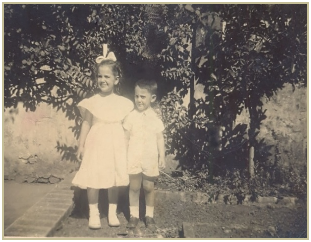
\includegraphics[width = 0.9\linewidth]{2/Reginaldo.png}
\caption{Reginaldo e eu por volta de 1950.}
\end{figure}

Uma das primeiras grandes sovas que levei, lembro, foi no Jardim da Infância porque havia, na escola, a atribuição semanal de uma “Medalha de Disciplina” aos que demonstravam melhor comportamento ao longo da semana e num sábado, excepcionalmente, eu não a trouxe para casa. 
Minha professora me deixara tomando conta dos meus vinte e poucos coleguinhas para dar uma escapadela, sabe-se lá para onde e um deles me pediu que deixasse a turma escrever na lousa. 
Com o discernimento a mim conferido pelos meus seis anos, achei que aquela seria uma boa forma de mantê-los ocupados. 
Não foi. 
Quando a professora retornou, havia giz para todo lado e um realizado e barulhento grupo de pirralhos tinha transformado não só a lousa como todas as paredes da sala numa exposição surrealista, sem que eu, impotente, conseguisse contê-los. 
Meu pai nem quis ouvir a história. 
Ainda hoje acho que a professora, D. Lídia, é que devia ter apanhado em meu lugar. 
 
Na família da minha mãe esse tratamento não existia. 
A menos que se levasse em consideração os beliscões e alfinetadas que marcavam os momentos relevantes dos sermões da Vó Didi às filhas adolescentes, enquanto lhes experimentava as costuras. 
Mamãe achava que ela reservava esse momento de propósito para os corretivos. O
Vô João, ao contrário, não só jamais se agastava como se apressava em protegê-las das tempestades maternas. 

Já na família do meu pai, o emprego da força física para dirimir questões de qualquer natureza era um valor muito apreciado. 
Vó Teresa, contava minha mãe, jactava-se de que seus filhos eram homens de resolver qualquer parada “com um soco só”. 

Um fato lembrado com divertida alacridade pelos irmãos Filpi, e exemplo amplamente divulgado do que acabo de relatar, dizia respeito a uma façanha perpetrada por um deles, o Tio Bepe, um rotundo peso-pesado de cento e trinta quilos, quando desconfiou que Tia Antonieta e Tia Glória, suas irmãs e noivas de dois irmãos, proprietários de uma vidraçaria, estavam sendo iludidas. 
Como a data do casamento ia sendo prorrogada ``ad infinitum'' pela família dos rapazes, ele decidiu tomar satisfação com os infelizes vidraceiros que, pálidos de terror, mal conseguiram entender o motivo da intempestiva visita, comunicado aos berros por cima do crepitar dos vidros pulverizados a murros por aquele búfalo ensandecido. 
Nem é preciso acrescentar que, com o estabelecimento, veio abaixo também o sonho das pobres moças de um dia se casarem. 

O castigo físico como recurso educativo era praticado com naturalidade e frequência entre os Filpi. 
Ouvi minhas tias aludirem, mais de uma vez, a uma bizarra norma pela qual, em crianças, quando um cometia uma falta passível de castigo, todos apanhavam para que um não caçoasse do outro. 
E papai lembrava com muito ressentimento uma passagem em que, muito pequeno ainda, distraíra-se observando formigas, deitado de bruços, espichado ao sol, ao invés de varrer o terreiro de café como lhe tinha sido ordenado.  
Sem dizer água vai, o avô Reginaldo, lá da varanda, fez estalar o comprido látego de conduzir charrete e desenhou-lhe um vergão em brasas ao comprido das costas. 
Revoltou-o demais o gesto tão violento quanto traiçoeiro. 
O que não o impediu de, ao crescer, acrescentar sua própria contribuição ao longo prontuário de brutalidades dos Filpi. 
Vovó Teresa nada ficava a dever ao marido no que diz respeito ao emprego da força como recurso disciplinar. 
Ao contrário, dado que Vovô se ausentava com freqüência, na maioria das vezes era a ela que cabia exemplar a numerosa prole. 
Mamãe contava ter presenciado uma cena em que tia Antonieta, a que mais ansiava por uma história de vida diferente daquela que levava em regime de semi-clausura, foi pedir à mãe permissão para continuar os estudos. 
Em resposta, recebeu tamanho safanão que perdeu o fôlego e a fala por longos e angustiantes segundos. 
E ela já era uma mocinha, a coitada.

Não é de admirar que os irmãos Filpi, incluídas aí as mulheres, uma vez adultos, fossem estimados e respeitados pelas numerosas qualidades de diligência, honestidade, generosidade, disponibilidade para com as necessidades do outro, mas igualmente temidos pela fúria demolidora que lhes podia brotar das entranhas quando enraivecidos.  
Naquele tempo, porém, no que toca aos machos da família, esta característica não chegava a causar grande escândalo porque encontrava certo amparo na mentalidade que predominava, como ainda predomina em alguns rincões da nossa sociedade, de que só pelo uso da força bruta um homem se legitima como tal. 
E o público feminino, não se pode negar, só recentemente começou a limitar seu entusiasmo por esse gênero de exibição. 
Mais de uma vez surpreendi uma expressão de orgulho na fisionomia da minha mãe quando meu pai se impunha pela força dos seus músculos. 
E ele nem precisava disso. 
Tinha estatura moral mais do que suficiente para conquistar naturalmente a admiração e o respeito de quantos o conheceram, inclusive e principalmente nossos, dos seus filhos. 

De qualquer maneira, no caso do meu pai, pelo menos, tenho certeza de que a necessidade de afirmar sua autoridade por esse meio era uma das injunções que o atormentavam. 
Tanto que, após cada um desses surtos de raiva primitiva e indomável, ele parecia consumir-se em arrependimento e buscava por todos os modos uma maneira de compensar a vítima: um presente, um passeio, um agrado qualquer. 
Mas jamais conseguiu reagir de outra maneira a uma situação em que se sentisse desafiado.

\begin{figure}[H]
\centering
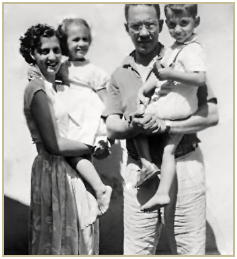
\includegraphics[width = 0.5\linewidth]{2/Familia.png}
\caption{Nossa família, no início dos anos 50.}
\end{figure}

Todos sabem que é contra o muro sólido do poder adulto que os jovens afiam seus dentes e garras. 
Seria preciso que meu pai fosse uma personalidade emocionalmente mais segura para suportar as investidas ditadas pela nossa imaturidade. 
Assombrava-o a possibilidade de cometer erros ou perder as rédeas na condução da família e na educação dos filhos. 
Porque, em nosso meio, esse seria o pior dos fracassos, o mais imperdoável, social ou pessoalmente falando. 
Ao contrário do que se ouve muitas vezes hoje, era opinião corrente que um filho desencaminhado expunha ao mundo a incompetência dos pais. 
Então, naquele tempo, mais que hoje em dia, à medida que a gente evoluía previsivelmente na direção da independência, os problemas em casa tendiam a aumentar na mesma proporção e o chamado “choque de gerações” sobrevinha com impacto terrível sobre as relações familiares. 
De alguma maneira, traumas a parte, esse conflito acabava por exercer uma força centrífuga de tal monta que raras vezes um jovem, depois de experimentá-la, desejava voltar para casa, a não ser depois que achasse um rumo na vida, ou seja, um diploma, um trabalho e até um casamento meio engatilhado. 
Essa podia não ser a forma mais adequada de pais promoverem a autonomia dos filhos, mas funcionava, sem sombra de dúvida. 
Os raros homens ou mulheres que permaneciam em casa, na dependência dos pais, além dos vinte e poucos anos, eram considerados indivíduos frustrados no seu desenvolvimento e olhados com um misto de piedade e estranheza.
As pessoas se perguntavam o que podia ter dado errado.  

Pode-se entender, neste contexto, a insegurança e as reações do meu pai, tendo sido ele próprio, além de tudo, um adolescente um tanto desajustado, sensível e difícil, que por pouco “não se perdeu por aí”, segundo contavam seus irmãos. 
Nele, como me acostumei a dizer, a rebeldia corcoveou até o fim sob a sela pesada da responsabilidade de homem de negócios e chefe de família. 
A repressão violenta exercida sobre nós, sobretudo os seus filhos mais velhos, hoje eu acredito, era também resultado de um esforço hercúleo para exorcizar sua própria inconformidade.

Aos catorze anos decidi que bastava. 
Quando num acesso de fúria meu pai levantou a mão para mim, encarei-o decidida a me defender, fosse como fosse. 
Acho que ele percebeu. Nunca mais repetiu o gesto. 
Paradoxalmente, entretanto, aquela manzorra pesada que tanto me apavorava quando se precipitava como aríete na minha direção, ficou na minha lembrança como a mesma que me comunicava tanta confiança e proteção quando se fechava, quente e firme, sobre minha pequena mão de criança.